\appendix
 
\subsection{Detailed Result Tables}\label{appendix:DetailedResults}

\begin{table*}[h!]
\centering
\caption{Sentence Boundary Detection Performance on Legal Texts by Dataset}
\label{tab:sbd-precision-performance}
\begin{tabular}{llrrrr}
\toprule
Dataset & Model & \textbf{Precision} & Chars/sec & F1 & Recall \\
\midrule
ALEA SBD Benchmark & NUPunkt & 0.918 & 10.00M & 0.842 & 0.778 \\
 & CharBoundary (large) & 0.637 & 518.06K & 0.727 & 0.847 \\
 & CharBoundary (medium) & 0.631 & 586.62K & 0.722 & 0.842 \\
 & CharBoundary (small) & 0.624 & 748.36K & 0.718 & 0.845 \\
 & NLTK Punkt & 0.537 & 9.09M & 0.646 & 0.811 \\
 & spaCy (lg) & 0.517 & 90.93K & 0.572 & 0.640 \\
 & spaCy (sm) & 0.516 & 96.51K & 0.573 & 0.644 \\
 & pySBD & 0.468 & 258.37K & 0.627 & 0.948 \\
\midrule
SCOTUS & CharBoundary (large) & 0.950 & 1.16M & 0.778 & 0.658 \\
 & CharBoundary (medium) & 0.938 & 1.36M & 0.775 & 0.661 \\
 & CharBoundary (small) & 0.926 & 1.35M & 0.773 & 0.664 \\
 & NUPunkt & 0.847 & 4.75M & 0.570 & 0.429 \\
 & spaCy (sm) & 0.825 & 110.13K & 0.761 & 0.706 \\
 & spaCy (lg) & 0.819 & 78.48K & 0.753 & 0.696 \\
 & pySBD & 0.799 & 284.47K & 0.817 & 0.835 \\
 & NLTK Punkt & 0.710 & 11.03M & 0.760 & 0.817 \\
\midrule
Cyber Crime & CharBoundary (large) & 0.968 & 698.33K & 0.853 & 0.762 \\
 & CharBoundary (medium) & 0.961 & 797.32K & 0.853 & 0.767 \\
 & CharBoundary (small) & 0.939 & 806.91K & 0.837 & 0.755 \\
 & NUPunkt & 0.901 & 11.29M & 0.591 & 0.439 \\
 & spaCy (sm) & 0.842 & 106.00K & 0.776 & 0.720 \\
 & pySBD & 0.831 & 216.49K & 0.833 & 0.835 \\
 & spaCy (lg) & 0.830 & 94.07K & 0.769 & 0.717 \\
 & NLTK Punkt & 0.748 & 10.40M & 0.782 & 0.819 \\
\midrule
BVA & NUPunkt & 0.987 & 14.77M & 0.608 & 0.440 \\
 & CharBoundary (large) & 0.963 & 991.14K & 0.881 & 0.813 \\
 & CharBoundary (medium) & 0.957 & 1.25M & 0.875 & 0.806 \\
 & CharBoundary (small) & 0.937 & 1.40M & 0.870 & 0.812 \\
 & pySBD & 0.795 & 217.58K & 0.857 & 0.929 \\
 & spaCy (sm) & 0.750 & 109.73K & 0.563 & 0.451 \\
 & spaCy (lg) & 0.720 & 114.30K & 0.554 & 0.450 \\
 & NLTK Punkt & 0.696 & 11.34M & 0.775 & 0.875 \\
\midrule
Intellectual Property & CharBoundary (large) & 0.954 & 791.24K & 0.890 & 0.834 \\
 & CharBoundary (medium) & 0.948 & 937.46K & 0.889 & 0.837 \\
 & CharBoundary (small) & 0.927 & 980.53K & 0.883 & 0.843 \\
 & NUPunkt & 0.912 & 13.01M & 0.595 & 0.442 \\
 & spaCy (sm) & 0.852 & 91.09K & 0.802 & 0.757 \\
 & spaCy (lg) & 0.839 & 92.16K & 0.792 & 0.749 \\
 & pySBD & 0.829 & 255.15K & 0.860 & 0.894 \\
 & NLTK Punkt & 0.724 & 10.65M & 0.781 & 0.847 \\
\bottomrule
\end{tabular}
\end{table*}

\begin{table*}[h!]
\centering
\caption{Memory Usage of Sentence Boundary Detection Methods}
\label{tab:memory-usage}
\begin{tabular}{lrrrr}
\toprule
\textbf{Tokenizer} & \textbf{Init (MB)} & \textbf{Tokenize (MB)} & \textbf{Bulk (MB)} & \textbf{Total (MB)} \\
\midrule
NUPunkt & 229.72 & 200.89 & 202.43 & 432.15 \\
NLTK Punkt & 285.39 & 174.21 & 174.25 & 459.63 \\
spaCy (sm) & 540.52 & 431.77 & 690.55 & 1231.07 \\
spaCy (lg) & 1060.02 & 1053.47 & 1307.31 & 2367.32 \\
pySBD & 1076.31 & 432.29 & 432.75 & 1509.06 \\
CharBoundary (small) & 518.77 & 506.91 & 507.07 & 1025.84 \\
CharBoundary (medium) & 948.56 & 948.66 & 948.20 & 1896.75 \\
CharBoundary (large) & 3402.06 & 2331.57 & 2331.87 & 5733.93 \\
\bottomrule
\end{tabular}
\end{table*}

\pagebreak

\subsection{Dataset Descriptions}
\label{appendix:Datasets}

We evaluated our approaches on five diverse legal datasets across two collections, summarized in Table~\ref{tab:sbd-precision-performance}. Table~\ref{tab:dataset-stats} provides detailed statistics for each dataset.

\begin{table*}[htbp]
\centering
\caption{Legal Dataset Statistics}
\label{tab:dataset-stats}
\begin{tabular}{lrrrr}
\toprule
Dataset & Examples & Sentences & Avg. Sentences/Doc & Avg. Sentence Length \\
\midrule
ALEA SBD Benchmark & 45155 & 171685 & 3.8 & 88.5 \\
SCOTUS & 20 & 6736 & 336.8 & 141.3 \\
Cyber Crime & 20 & 8293 & 414.6 & 117.5 \\
BVA & 20 & 3683 & 184.2 & 125.8 \\
Intellectual Property & 20 & 7187 & 359.4 & 128.3 \\
\bottomrule
\end{tabular}
\end{table*}



\subsubsection{ALEA SBD Benchmark}
The ALEA SBD Benchmark is a comprehensive dataset of legal documents with sentence boundary annotations using the \texttt{<|sentence|>} delimiter format. This dataset was constructed by synthetically annotating random samples from the KL3M Dataset using GPT-4o to generate initial annotations, followed by Claude 3.7 Sonnet to judge and correct the boundaries.

\begin{itemize}
    \item Contains 45,155 documents with 171,685 sentence boundaries (training partition)
    \item Average of 3.8 sentences per document with mean sentence length of 88.5 characters 
    \item Diverse legal content including regulatory filings, case law, and contracts
    \item Extensive coverage of legal-specific text patterns including citations, abbreviations, and numbered lists
\end{itemize}

The dataset is publicly available on Hugging Face Datasets and GitHub, providing a high-quality benchmark for evaluating sentence boundary detection in legal text.

\begin{center}
\url{https://huggingface.co/datasets/alea-institute/alea-legal-benchmark-sentence-paragraph-boundaries}
\end{center}

\subsubsection{MultiLegalSBD Collection}
The MultiLegalSBD collection introduced by Brugger et al. \cite{multilegalSBD} consists of four specialized legal subdomain datasets with character-span annotations that identify exact positions of sentence boundaries:

\begin{itemize}
    \item \textbf{U.S. Supreme Court opinions (SCOTUS):} 20 documents with 6,736 sentences (336.8 per document)
    \begin{itemize}
        \item Characterized by formal legal language, complex citations, and long multi-clause sentences
        \item Average sentence length of 141.3 characters
    \end{itemize}
    
    \item \textbf{Cyber Crime case law (Cyber Crime):} 20 documents with 8,293 sentences (414.6 per document)
    \begin{itemize}
        \item Features technical terminology and specialized citations to digital evidence
        \item Average sentence length of 117.5 characters
    \end{itemize}
    
    \item \textbf{Board of Veterans Appeals decisions (BVA):} 20 documents with 3,683 sentences (184.2 per document)
    \begin{itemize}
        \item Structured formatting, frequent abbreviations, and specialized veterans' benefits terminology
        \item Average sentence length of 125.8 characters
    \end{itemize}
    
    \item \textbf{Intellectual property cases (IP):} 20 documents with 7,187 sentences (359.4 per document)
    \begin{itemize}
        \item Contains technical descriptions, complex citations to prior art, and specialized IP terminology
        \item Average sentence length of 128.3 characters
    \end{itemize}
\end{itemize}

The MultiLegalSBD collection is part of a larger multilingual dataset containing over 130,000 annotated sentences across six languages. For our evaluation, we focused on the English legal subdomain datasets.

\subsection{NUPunkt Algorithm}
\label{appendix:NUPunkt}

NUPunkt extends the original Punkt algorithm \cite{kiss2006unsupervised} with specialized optimizations for legal text. It operates on a fully unsupervised basis, requiring no labeled training data, making it particularly suitable for rapid deployment across diverse legal domains. The algorithm is implemented as a pure Python library with zero external dependencies, ensuring easy integration across environments.

For a comprehensive overview of the algorithm, implementation details, and source code, we refer readers to the official repository:

\begin{center}
\url{https://github.com/alea-institute/NUPunkt}
\end{center}

\subsection{Key Features and Optimizations}

NUPunkt includes the following key components and optimizations specifically for legal text:

\begin{itemize}
\item \textbf{Legal-Specific Abbreviation Dictionary:} A comprehensive collection of over 4,000 abbreviations commonly found in legal and financial documents.
\item \textbf{Citation Pattern Recognition:} Specialized regular expressions to preserve legal citation formats.
\item \textbf{Hierarchical Structure Recognition:} Improved handling of enumerated lists and section headers.
\item \textbf{Optimized Implementation:} Extensive use of caching, pre-compiled patterns, and fast path processing.
\end{itemize}

\subsection{Performance Characteristics}

The NUPunkt algorithm demonstrates the following performance metrics:
\begin{itemize}
\item \textbf{Processing Speed:} Typically 30-35 million characters per second on standard hardware
\item \textbf{Fast Path Optimization:} Up to 1.4 billion characters per second for texts without sentence boundaries
\item \textbf{Memory Usage:} Minimal memory footprint due to pure Python implementation
\item \textbf{Initialization Time:} Sub-second startup time with pre-trained model
\end{itemize}

\subsection{CharBoundary Algorithm}
\label{appendix:CharBoundary}

CharBoundary implements a fundamentally different approach to sentence boundary detection, operating at the character level rather than the token level. Unlike NUPunkt's unsupervised approach, CharBoundary employs supervised machine learning to classify potential boundary positions based on local character context and legally-relevant features. This approach enables more nuanced decision-making specifically optimized for legal domain text.

For complete implementation details, model architecture, and source code, we refer readers to the official repository:

\begin{center}
\url{https://github.com/alea-institute/CharBoundary}
\end{center}

\subsection{Key Features}

The key innovations of the CharBoundary approach include:

\begin{itemize}
\item \textbf{Character-Level Analysis:} Uses a sliding window approach to extract features from surrounding character context.
\item \textbf{Machine Learning Classification:} Employs a Random Forest model to distinguish between sentence boundaries and non-boundaries.
\item \textbf{Legal-Specific Feature Detection:} Specialized features for legal text challenges including abbreviation detection, citation recognition, and list structure preservation.
\item \textbf{Configurable Precision/Recall:} Provides runtime-adjustable probability thresholds for fine-tuning performance to specific requirements.
\end{itemize}

\subsection{Model Variants}

Three pre-trained models offer different performance profiles:

\begin{itemize}
\item \textbf{Small Model:} 32 trees, 5-character window, optimized for speed (~748,000 chars/sec)
\item \textbf{Medium Model:} 64 trees, 7-character window, balanced performance (~586,000 chars/sec)
\item \textbf{Large Model:} 256 trees, 9-character window, maximizes accuracy (~518,000 chars/sec)
\end{itemize}

\begin{table}[htbp!]
\centering
\caption{CharBoundary Model Size Comparison}
\label{tab:charboundary-model-size}
\begin{tabular}{lrrrr}
\toprule
\textbf{Model} & \textbf{SKOPS Size} & \textbf{ONNX Size} & \textbf{Memory Usage} & \textbf{Throughput} \\
\textbf{Variant} & \textbf{(MB)} & \textbf{(MB)} & \textbf{(MB)} & \textbf{(chars/sec)} \\
\midrule
Small & 3.0 & 0.5 & 1,025.84 & $\sim$748K \\
Medium & 13.0 & 2.6 & 1,896.75 & $\sim$586K \\
Large & 60.0 & 13.0 & 5,733.93 & $\sim$518K \\
\bottomrule
\end{tabular}
\end{table}

\subsection{Performance Optimizations}

Major performance optimizations include:

\begin{itemize}
\item \textbf{Selective Processing:} Focuses only on potential boundary positions (typically under 5\% of characters)
\item \textbf{ONNX Runtime Integration:} Enables optimized execution with 1.1x-2.1x faster inference
\item \textbf{Parallel Processing:} Automatically partitions large documents for parallel processing
\item \textbf{Hierarchical Caching:} Multi-level caching system for frequent patterns and decisions
\end{itemize}

\subsection{Performance Characteristics}

\begin{itemize}
\item \textbf{Throughput:} 377,000-600,000 characters/second depending on model size
\item \textbf{Memory Efficiency:} Scales with chunk size rather than total document length
\item \textbf{Algorithmic Complexity:} $O(t \times f)$ where $t$ is the number of potential boundary positions and $f$ is the number of features
\item \textbf{Latency:} Optimized for documents of all sizes with parallel processing for large texts
\end{itemize}

\subsection{Interactive Demonstration}
\label{appendix:demo}

To facilitate adoption and further research, we provide an interactive web demonstration of our sentence boundary detection tools at \url{https://sentences.aleainstitute.ai/}. This demonstration allows users to:

\begin{itemize}
\item Compare multiple sentence boundary detection algorithms (NLTK, spaCy, pySBD, NUPunkt, and CharBoundary) side-by-side
\item Adjust the probability threshold for the CharBoundary model to explore precision-recall tradeoffs
\item Test algorithms on custom legal text or pre-loaded examples
\item Generate shareable links to specific analyses for collaboration
\end{itemize}

The interactive nature of this tool provides both researchers and practitioners with a practical way to evaluate the performance of different sentence boundary detection approaches on their specific legal text corpus without requiring local installation. Additionally, all source code and data needed to replicate the experiments and results in this paper are available at \url{https://github.com/alea-institute/legal-sentence-paper}.

\subsection{Additional Figures}
\label{appendix:Figures}

\begin{figure*}[htbp]
\centering
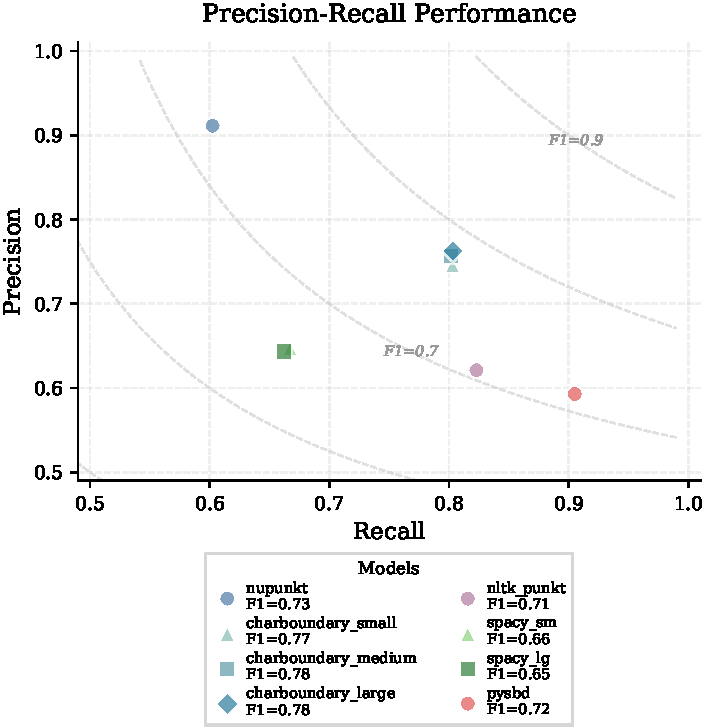
\includegraphics[width=0.7\textwidth]{figures/precision_recall.pdf}
\caption{Precision vs. recall comparison across models.}
\label{fig:precision_recall_tradeoff}
\end{figure*}

\begin{figure*}[htbp]
    \centering
    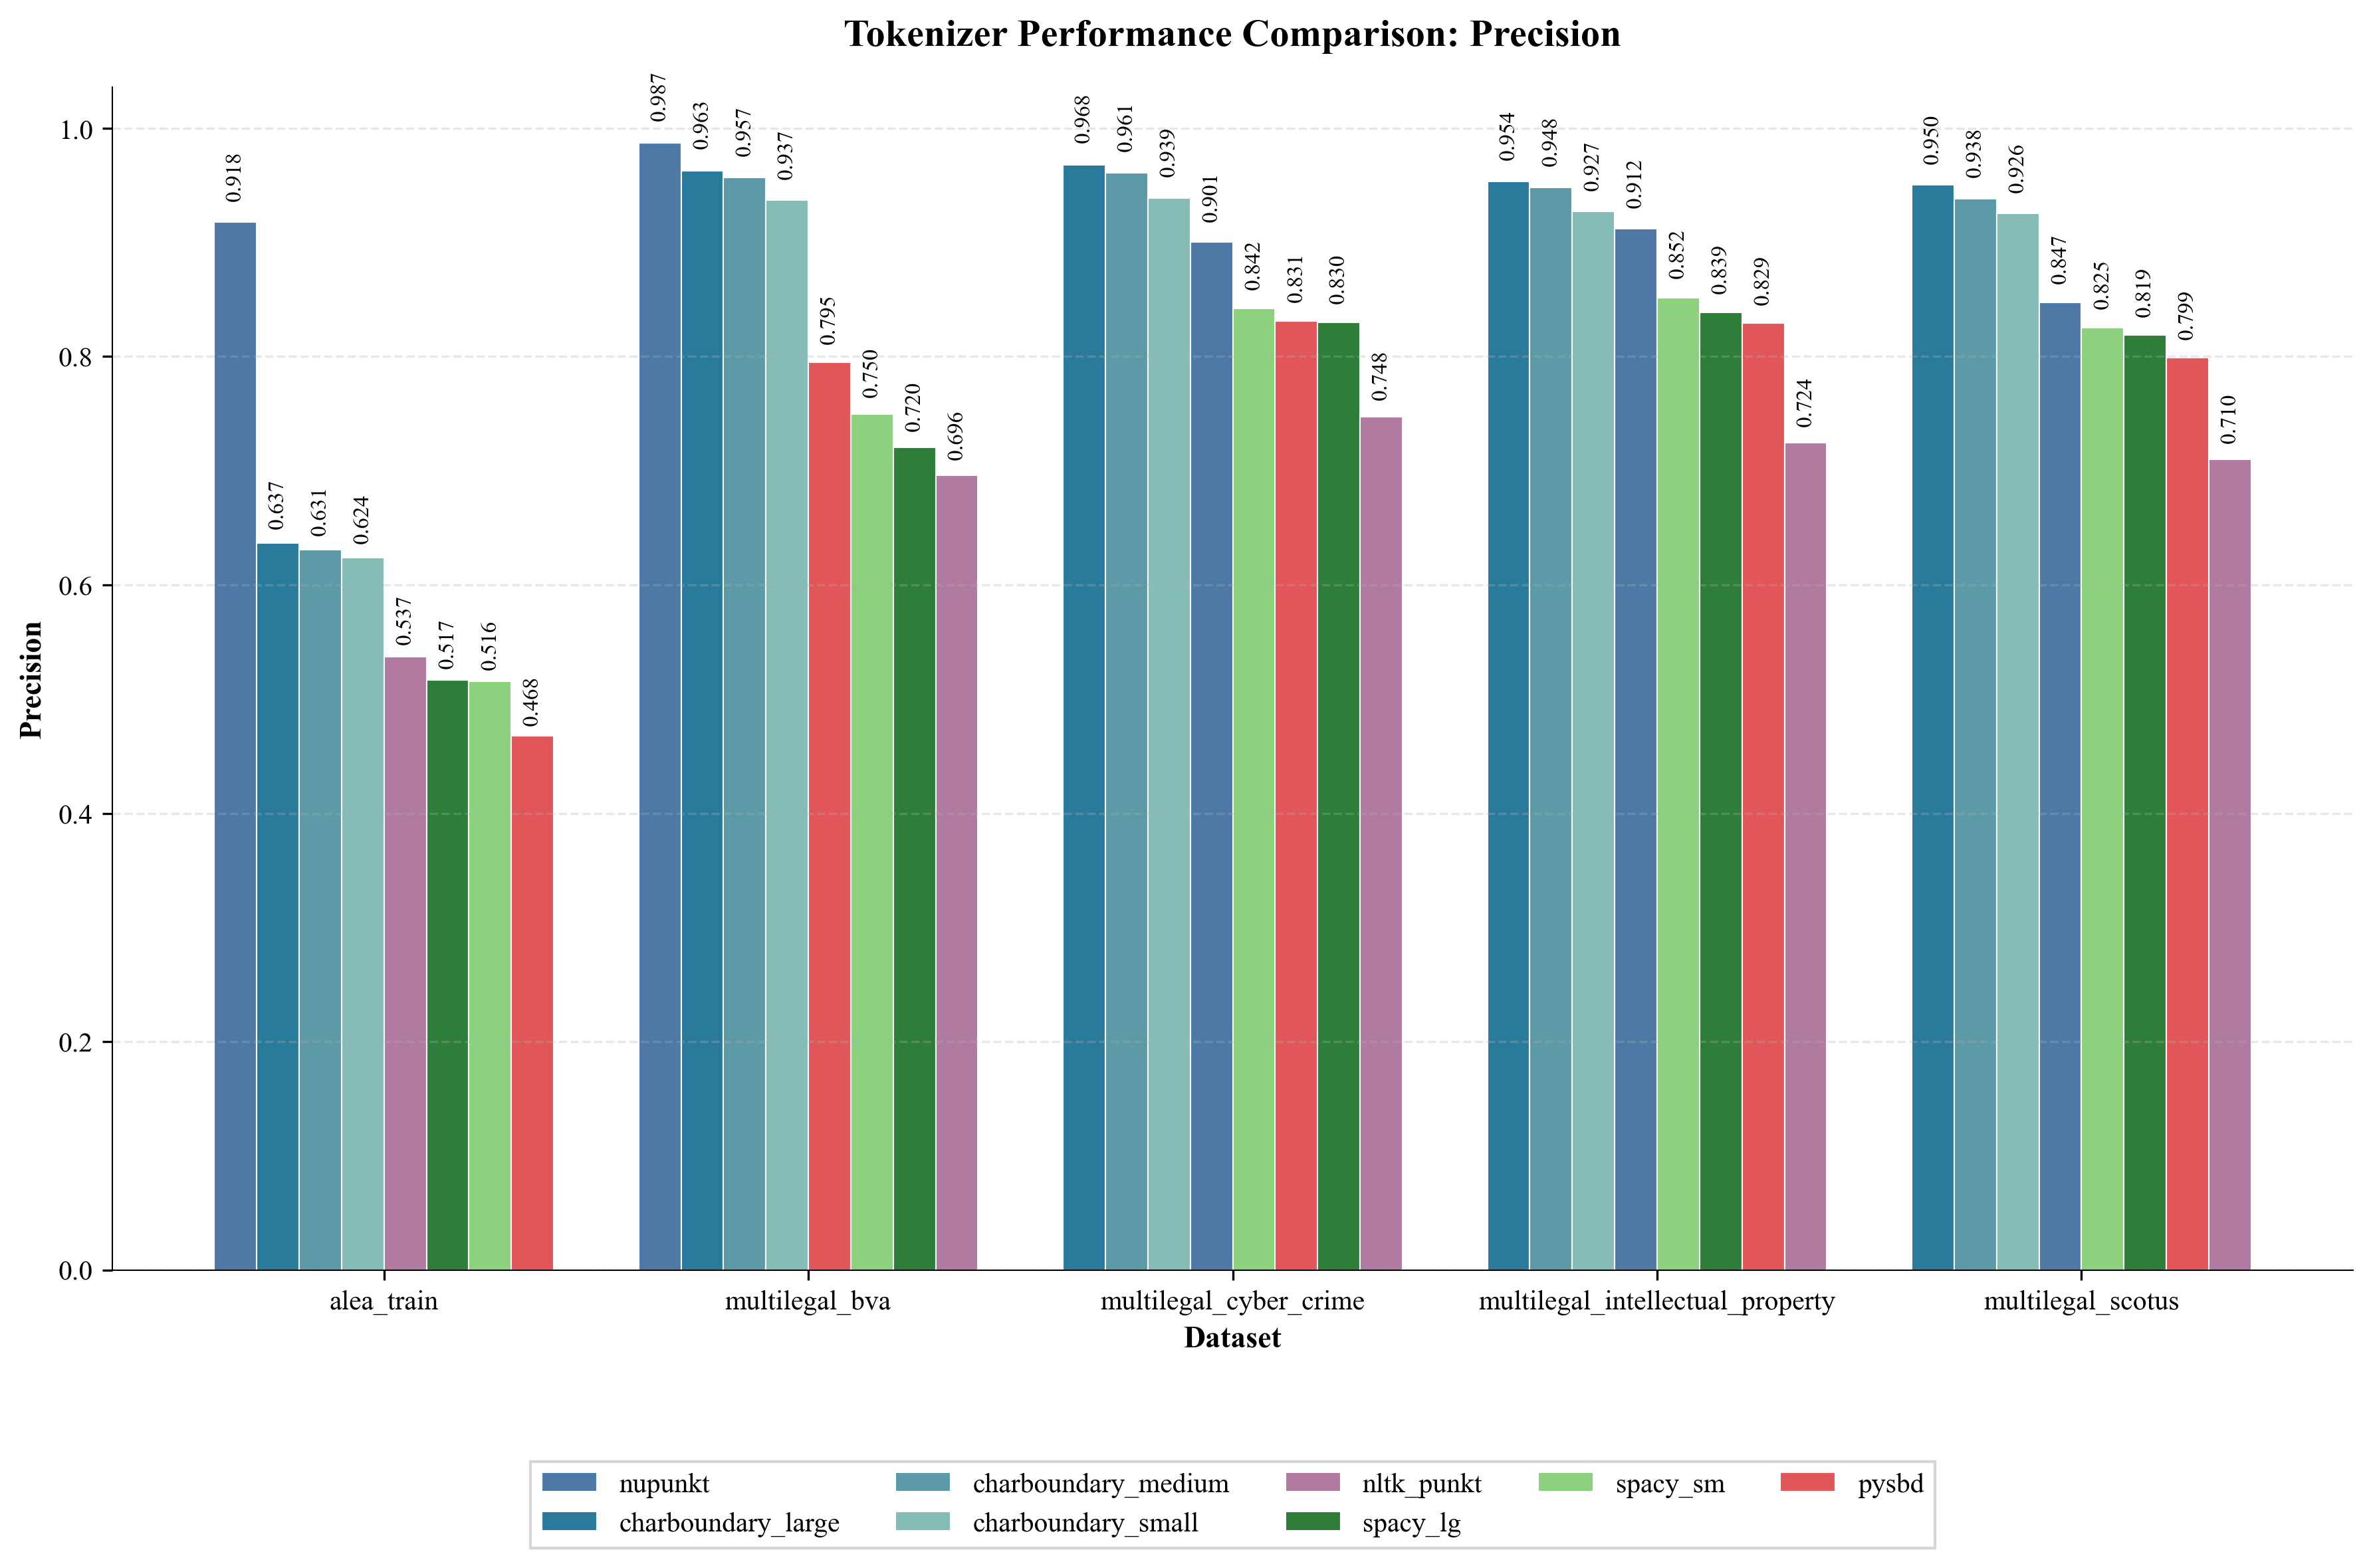
\includegraphics[width=0.75\textwidth]{figures/precision.png}
    \caption{Precision comparison across models and datasets.}
    \label{fig:precision_comparison}
\end{figure*}

\begin{figure*}[htbp]
    \centering
    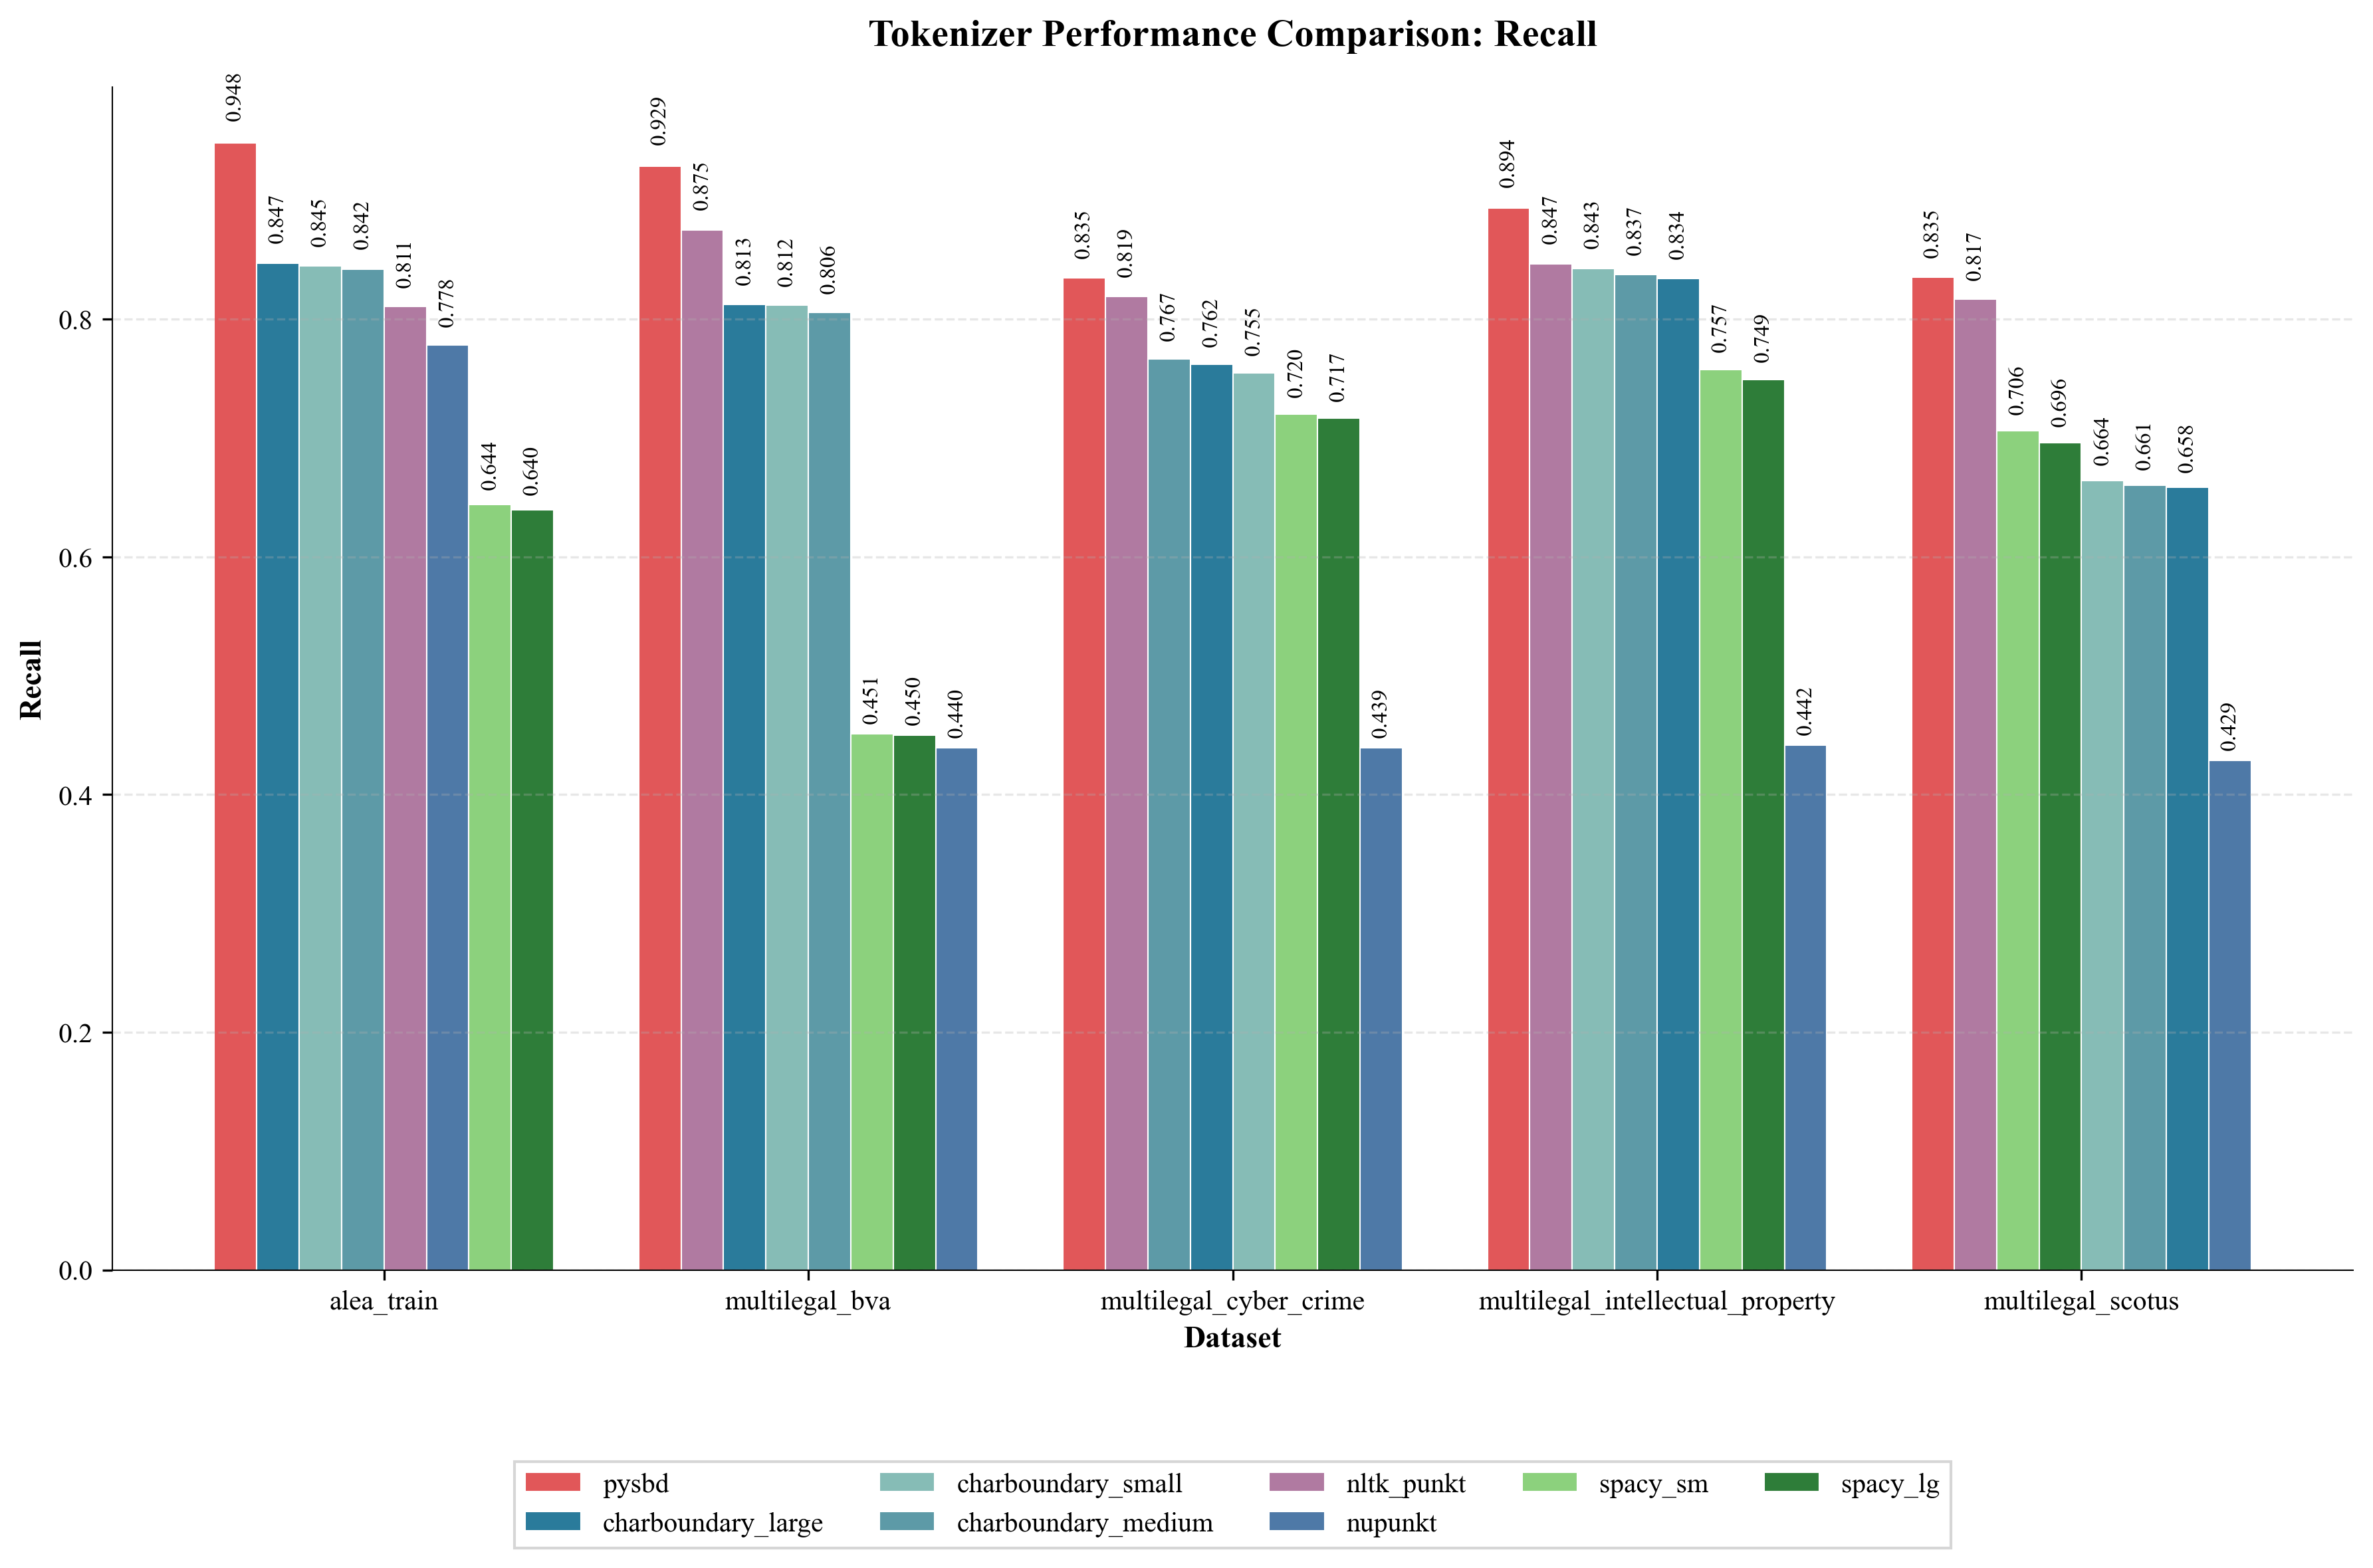
\includegraphics[width=0.75\textwidth]{figures/recall.png}
    \caption{Recall comparison across models and datasets.}
    \label{fig:recall_comparison}
\end{figure*}

\begin{figure*}[htbp]
    \centering
    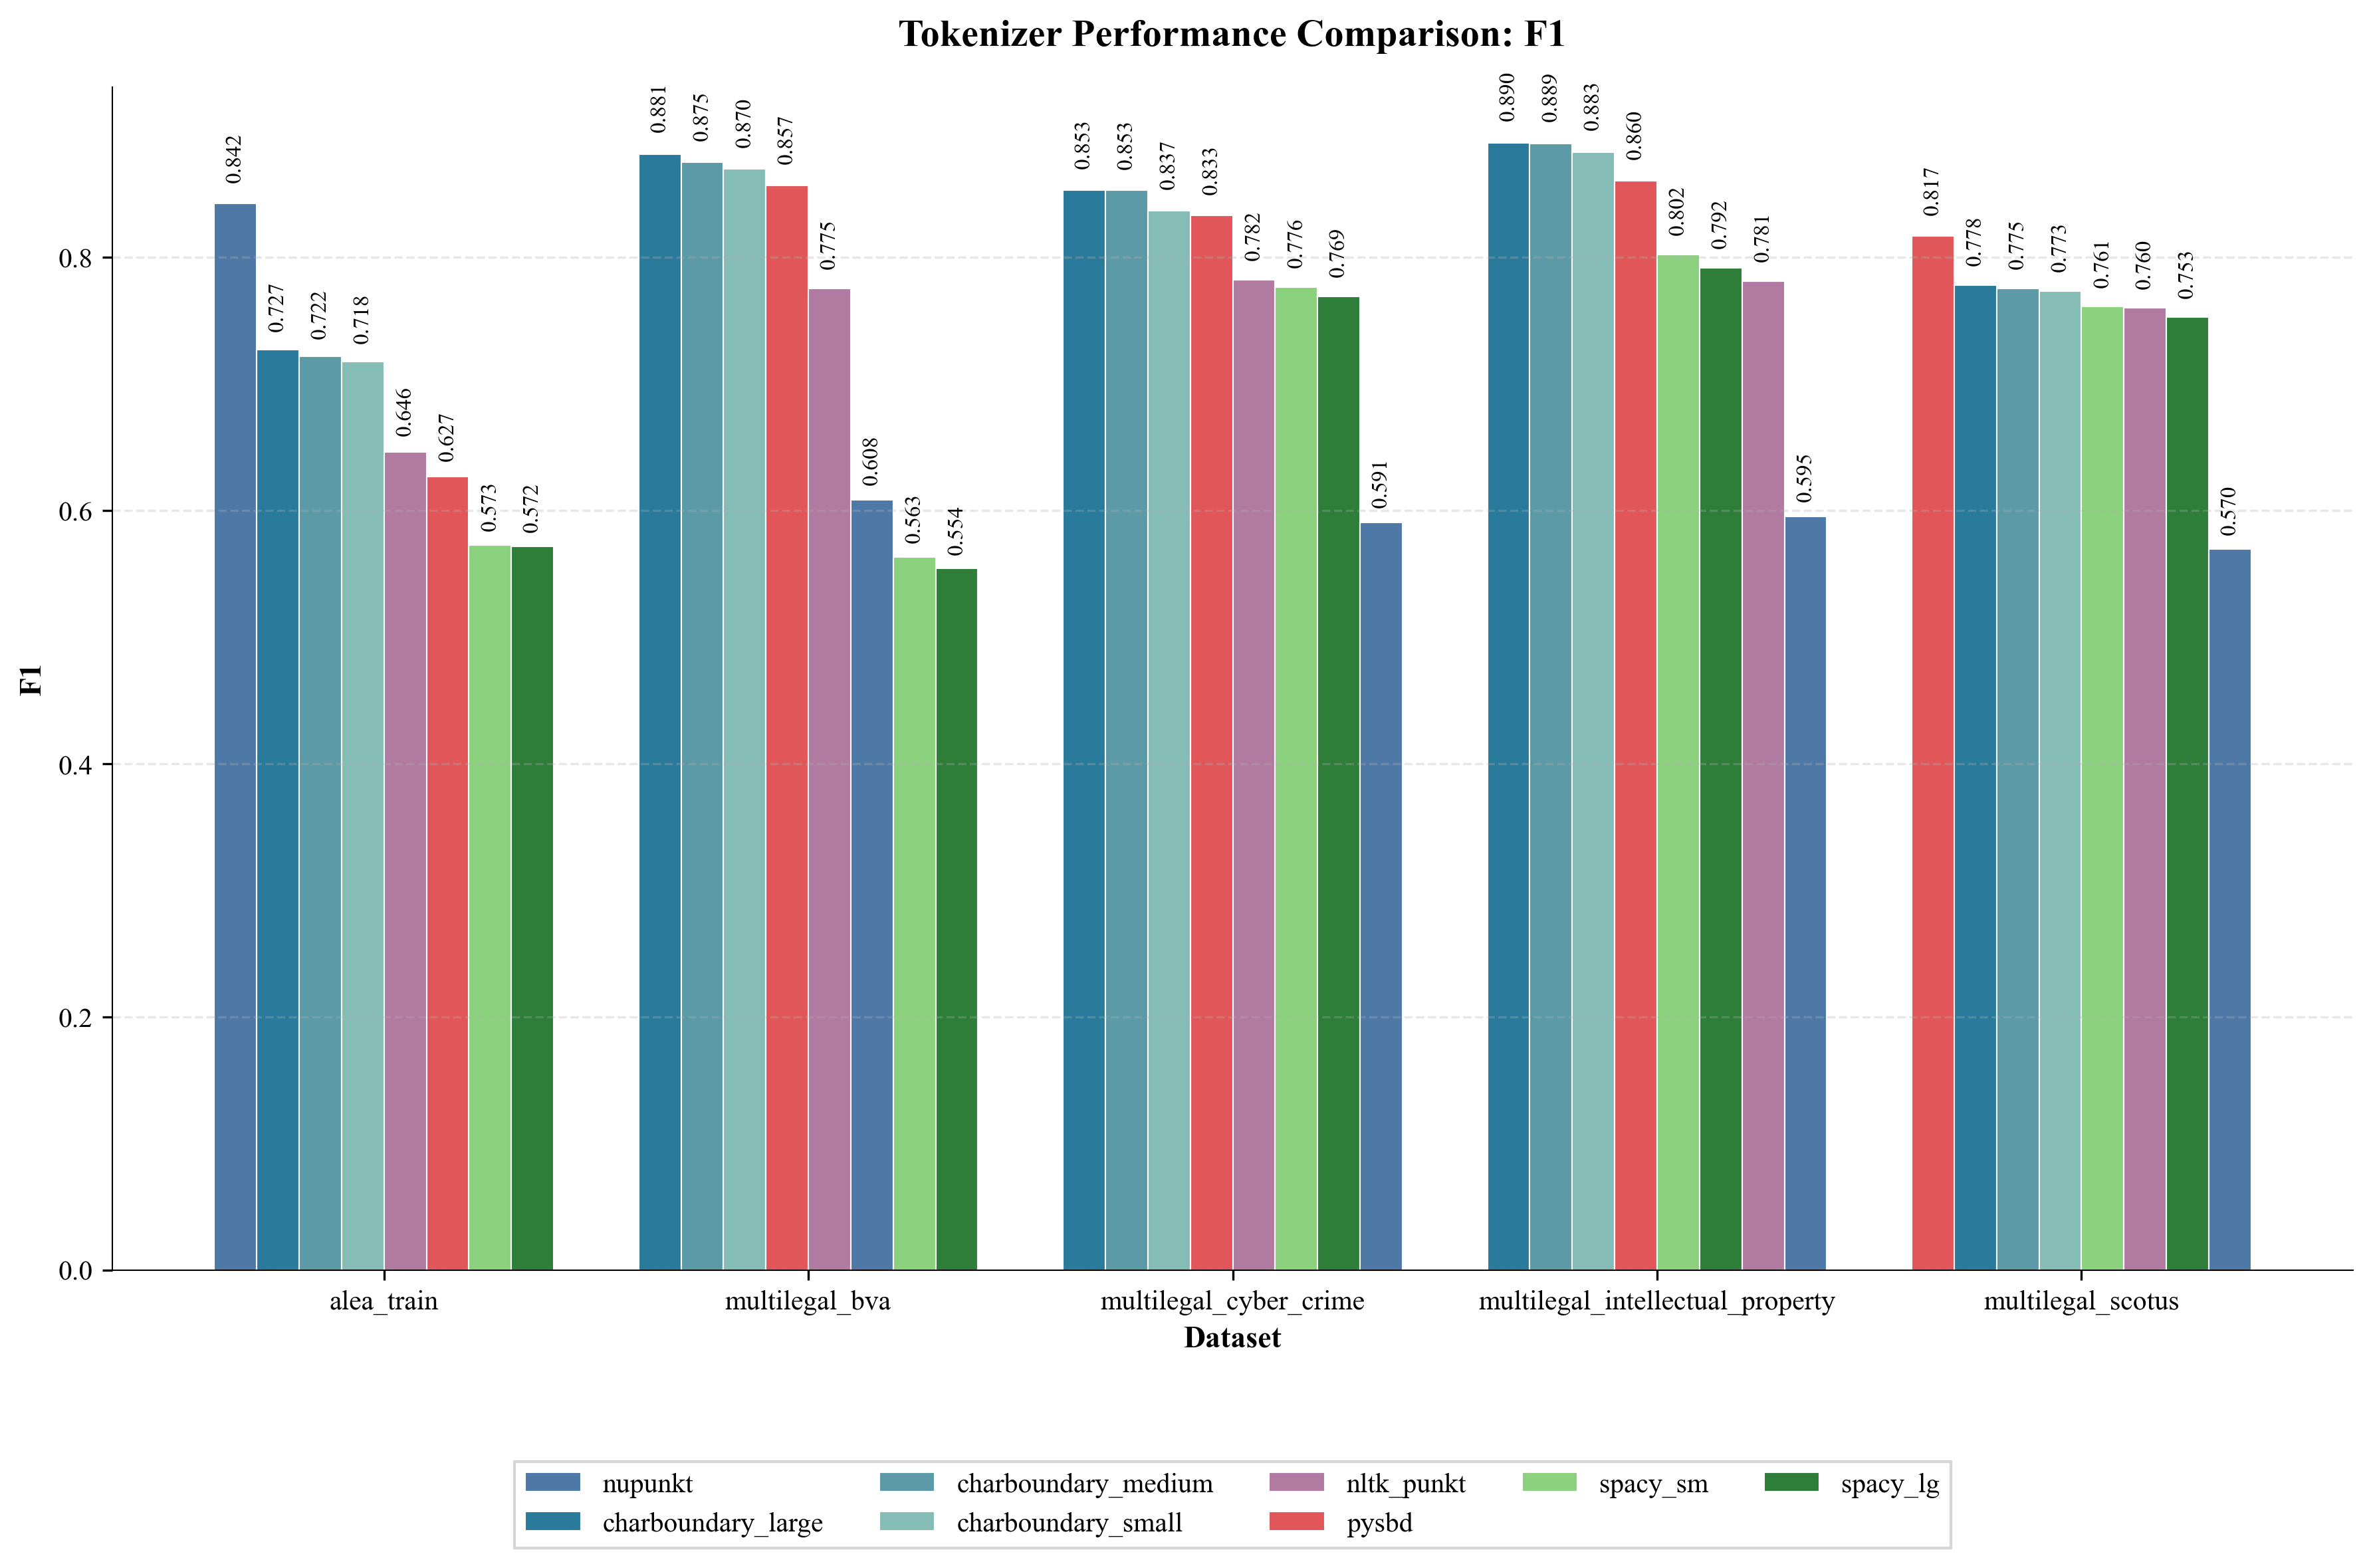
\includegraphics[width=0.75\textwidth]{figures/f1.png}
    \caption{F1 score comparison across models and datasets.}
    \label{fig:f1_comparison}
\end{figure*}

